\begin{figure}[h]
    \centering
    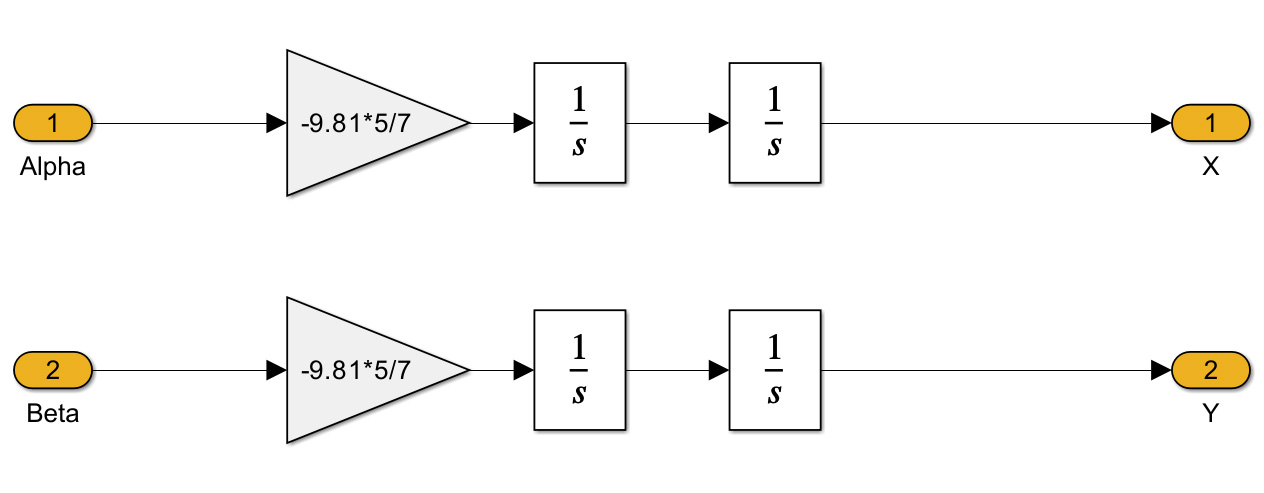
\includegraphics[width=1\linewidth]{Figures/chapter03/Linear_BPS_Simulink_Model_inTransferFunction.jpg}
    \caption{Linear simulation model of the Ball and Plate System in a transfer function form}

\end{figure}
\begin{figure}
    \centering
    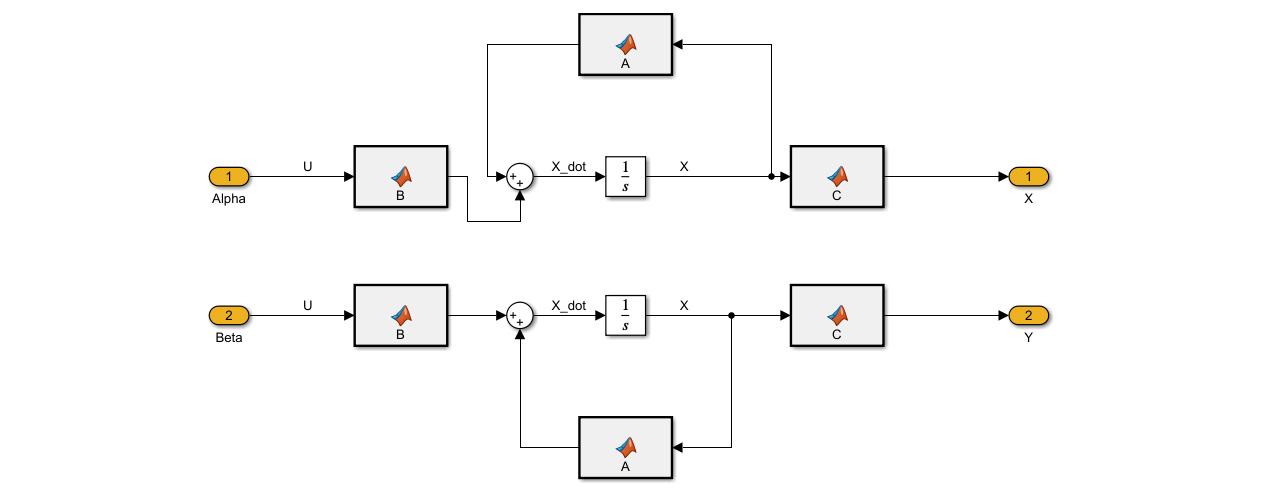
\includegraphics[width=1\linewidth]{Figures/chapter03/Linear_BPS_Simulink_Model_inStateSpace.jpg}
    \caption{Linear simulation model of the Ball and Plate System in state-space form}
\end{figure}

\begin{sidewaysfigure}
\centering
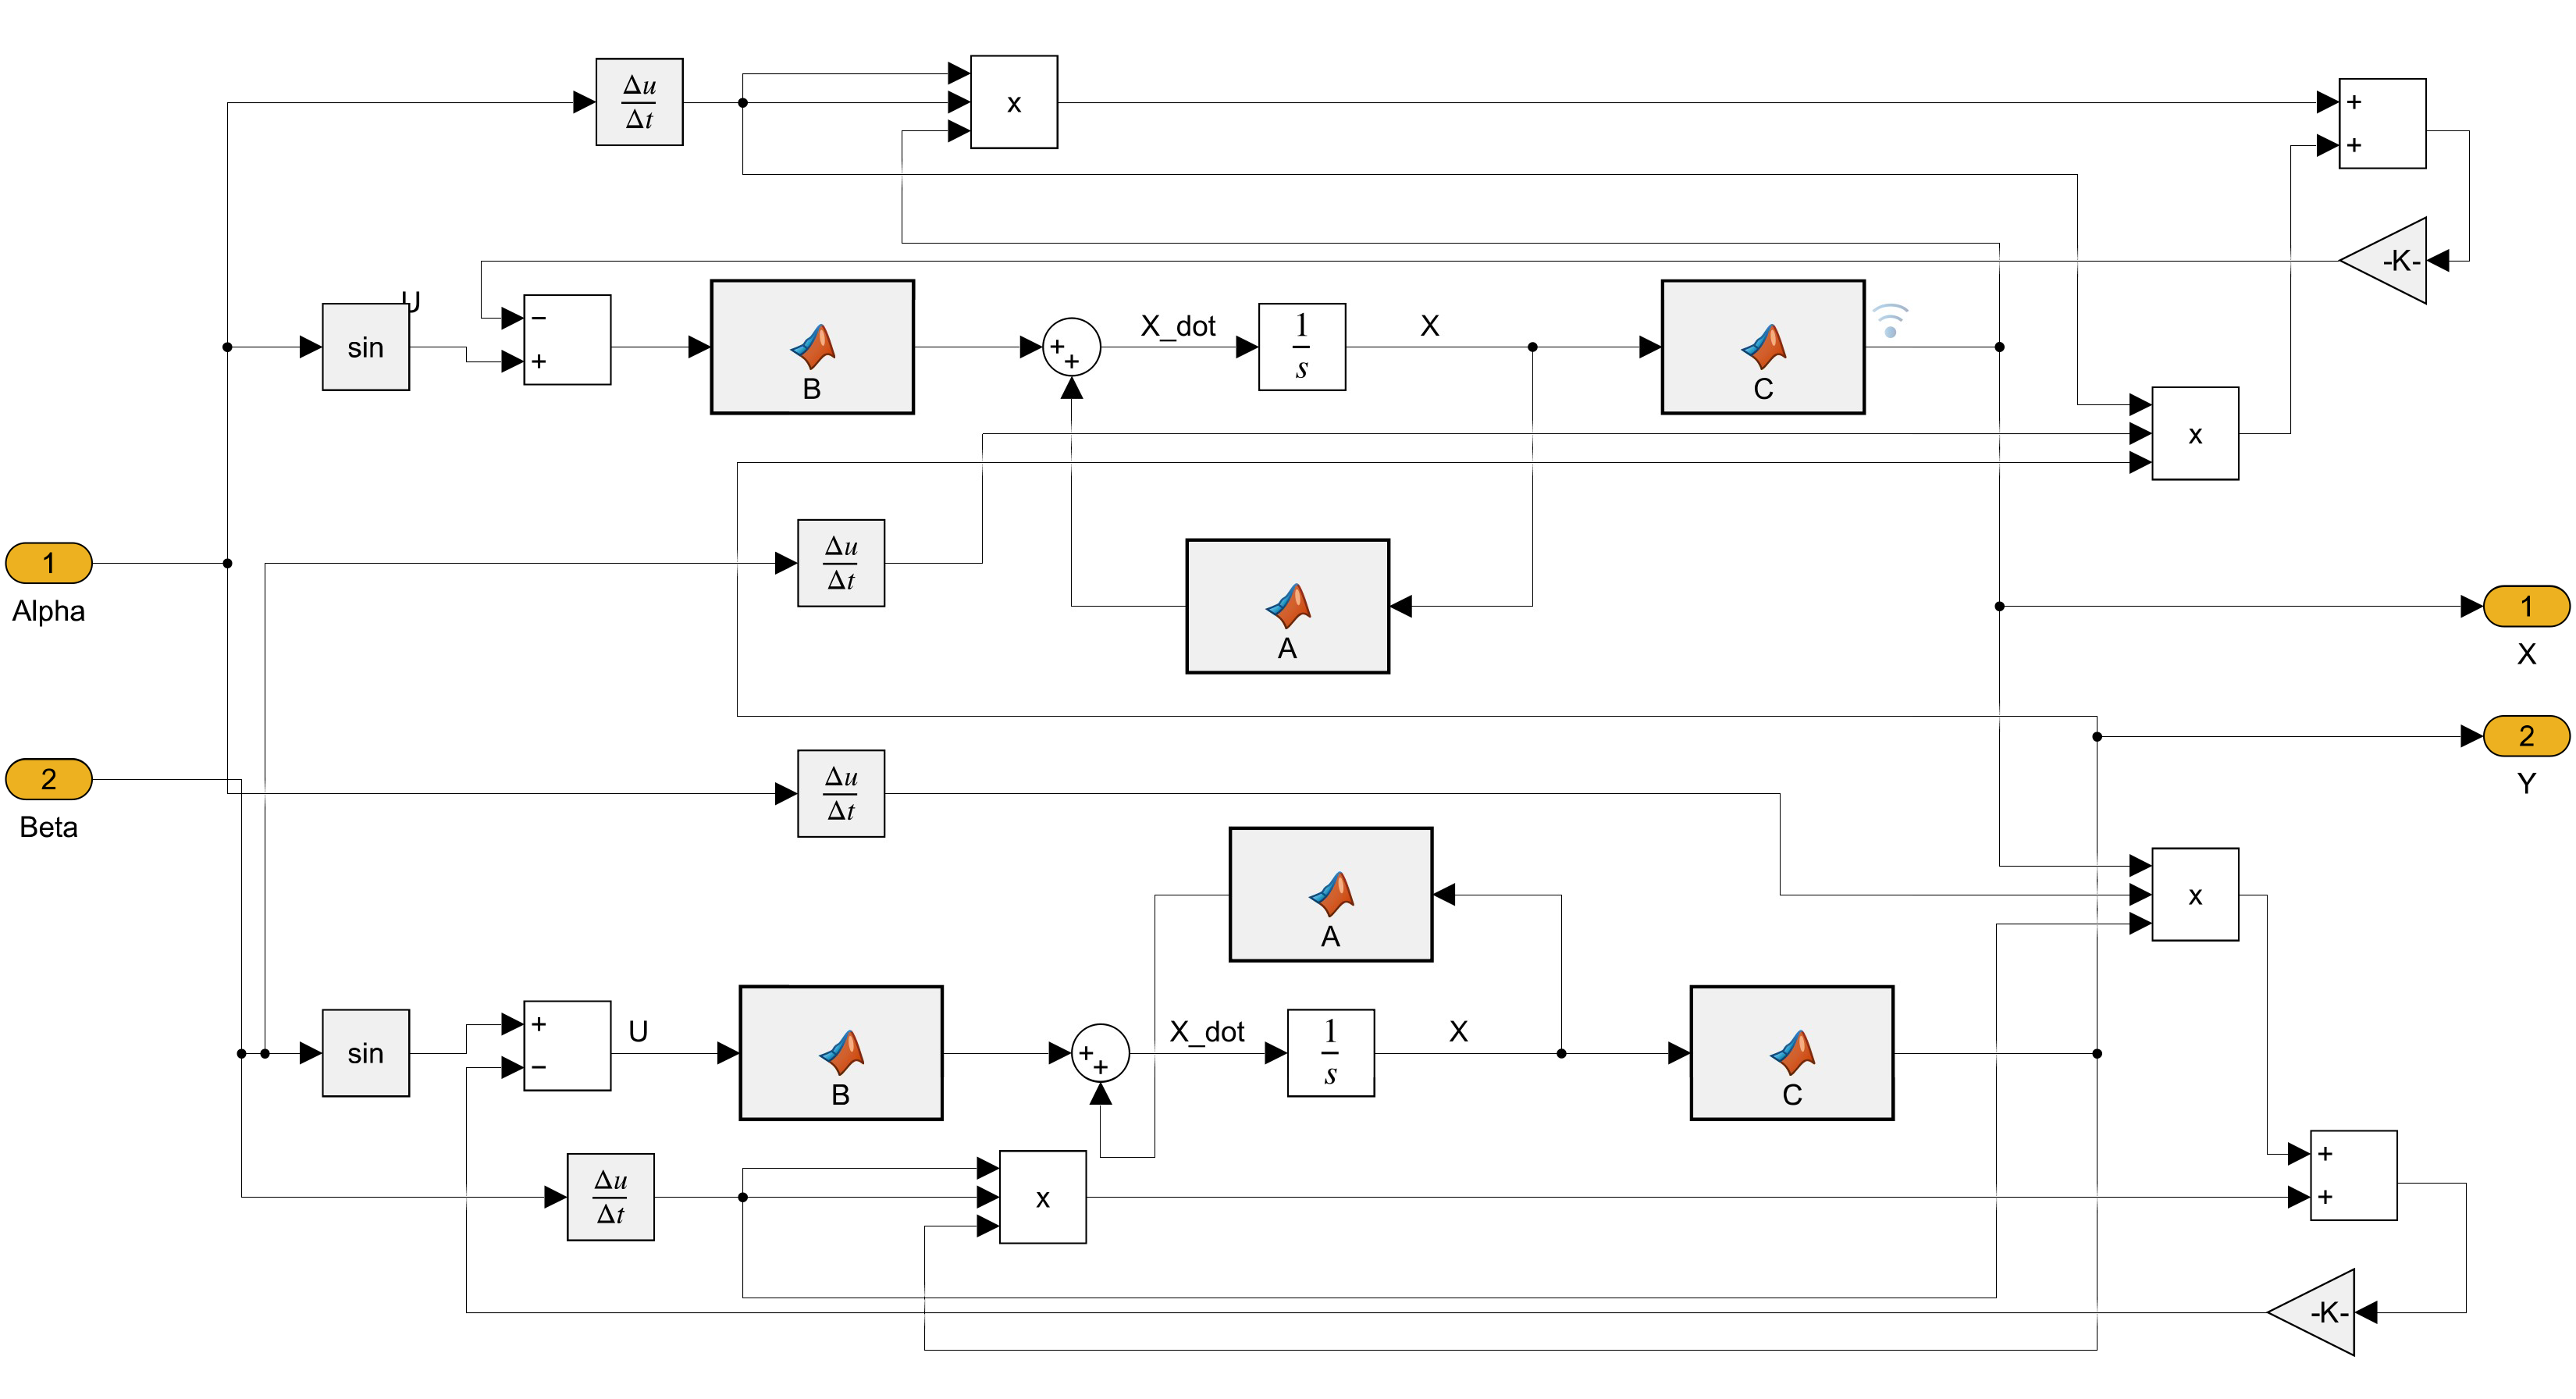
\includegraphics[width=0.95\textheight]{Figures/chapter03/nonlinear.png}
\caption{Approximated representation of the non-linear BPS dynamics in a Simulink model}
\label{fig:IMs matrix correlation}
\end{sidewaysfigure}

\begin{sidewaysfigure}
\centering
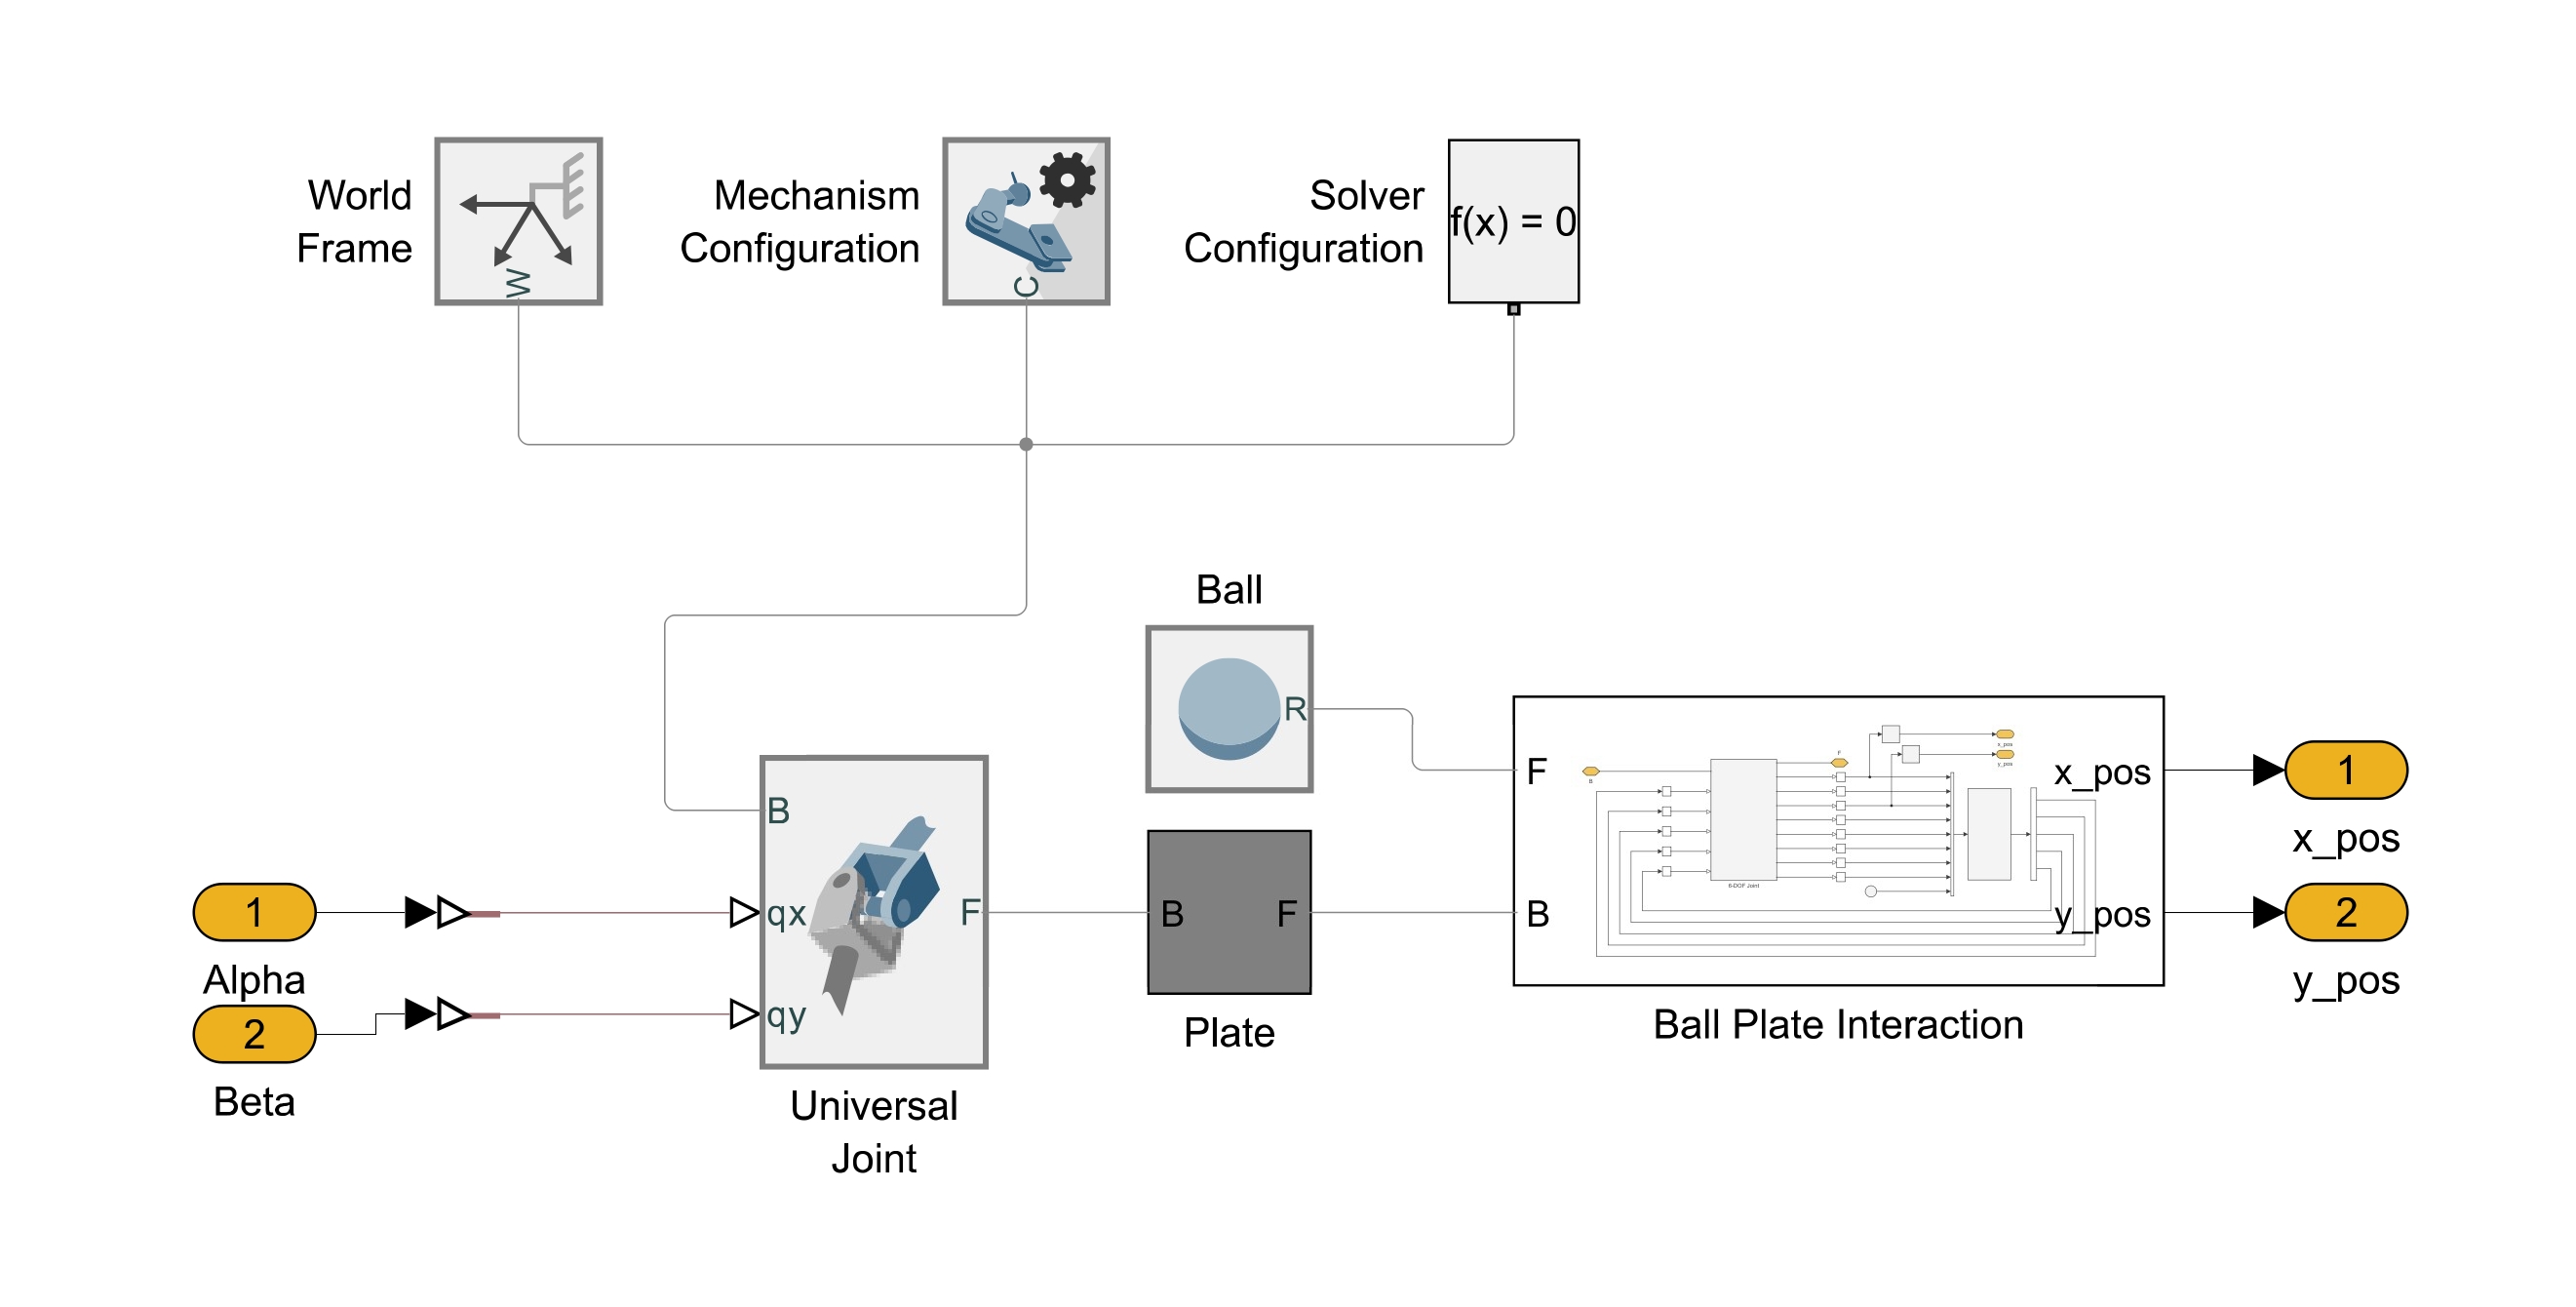
\includegraphics[width=0.95\textheight]{Figures/chapter03/simscape.png}
\caption{Dynamic simulation of the non-linear Ball and Plate System using Simscape}
\label{fig:IMs matrix correlation}
\end{sidewaysfigure}

\begin{sidewaysfigure}
\centering
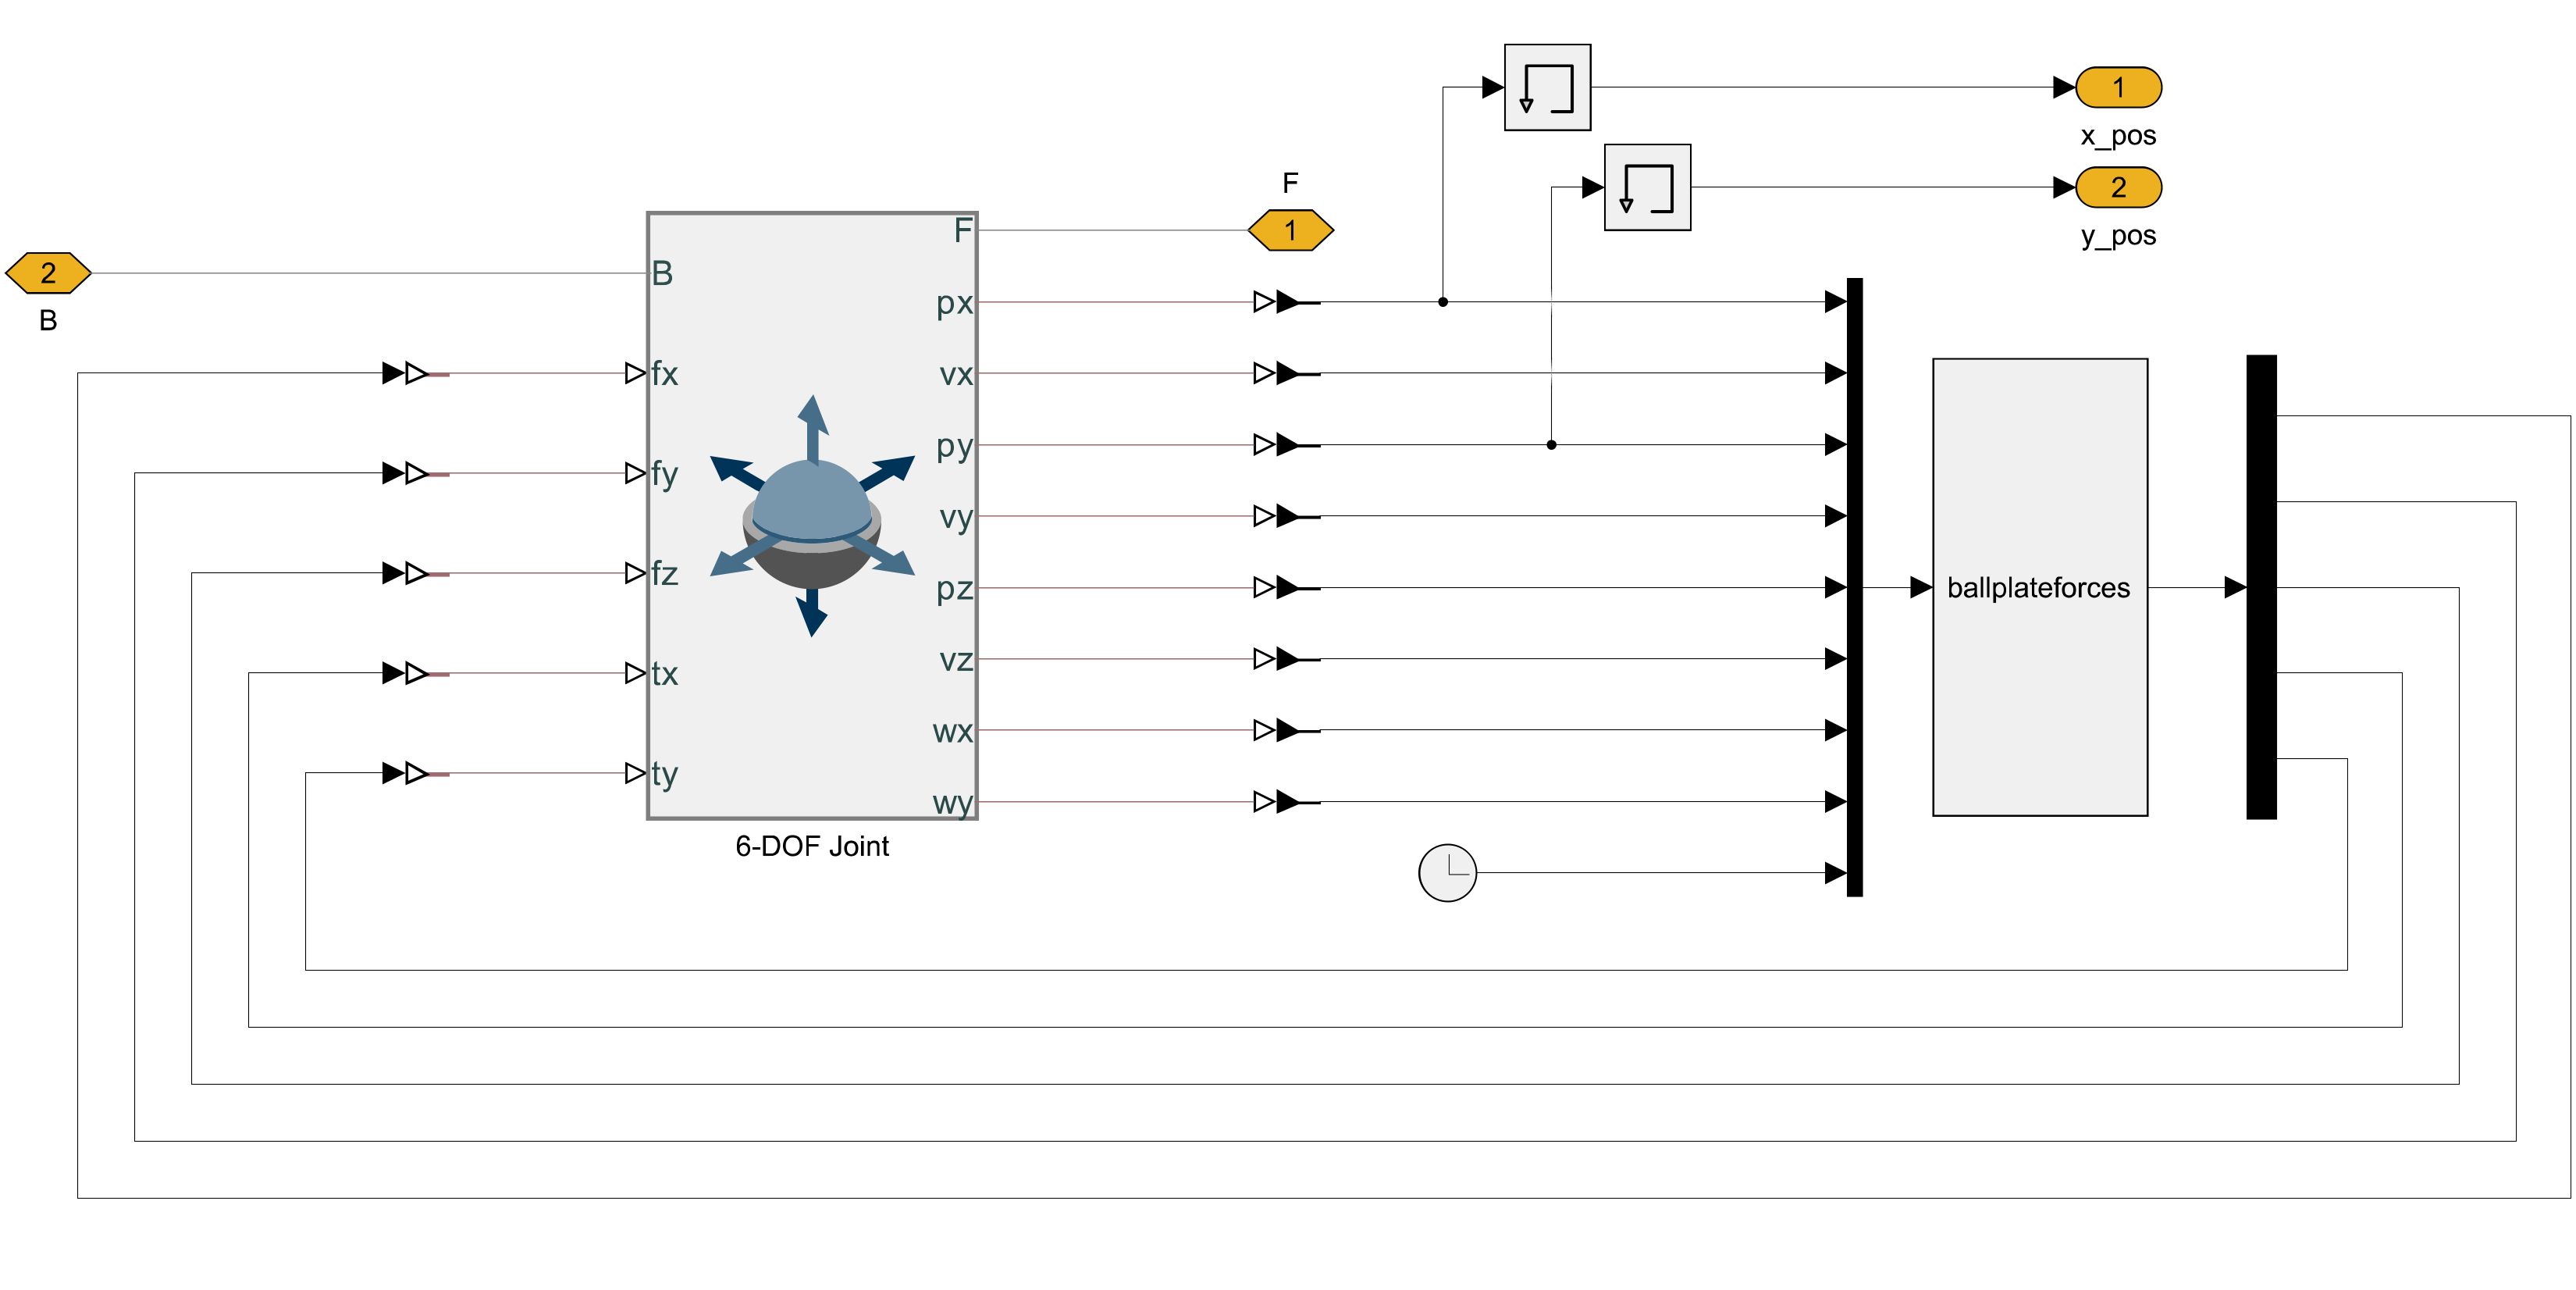
\includegraphics[width=0.95\textheight]{Figures/chapter03/BPinteration.png}
\caption{BPS interaction subsystem}
\label{fig:IMs matrix correlation}
\end{sidewaysfigure}

\begin{sidewaysfigure}
\centering
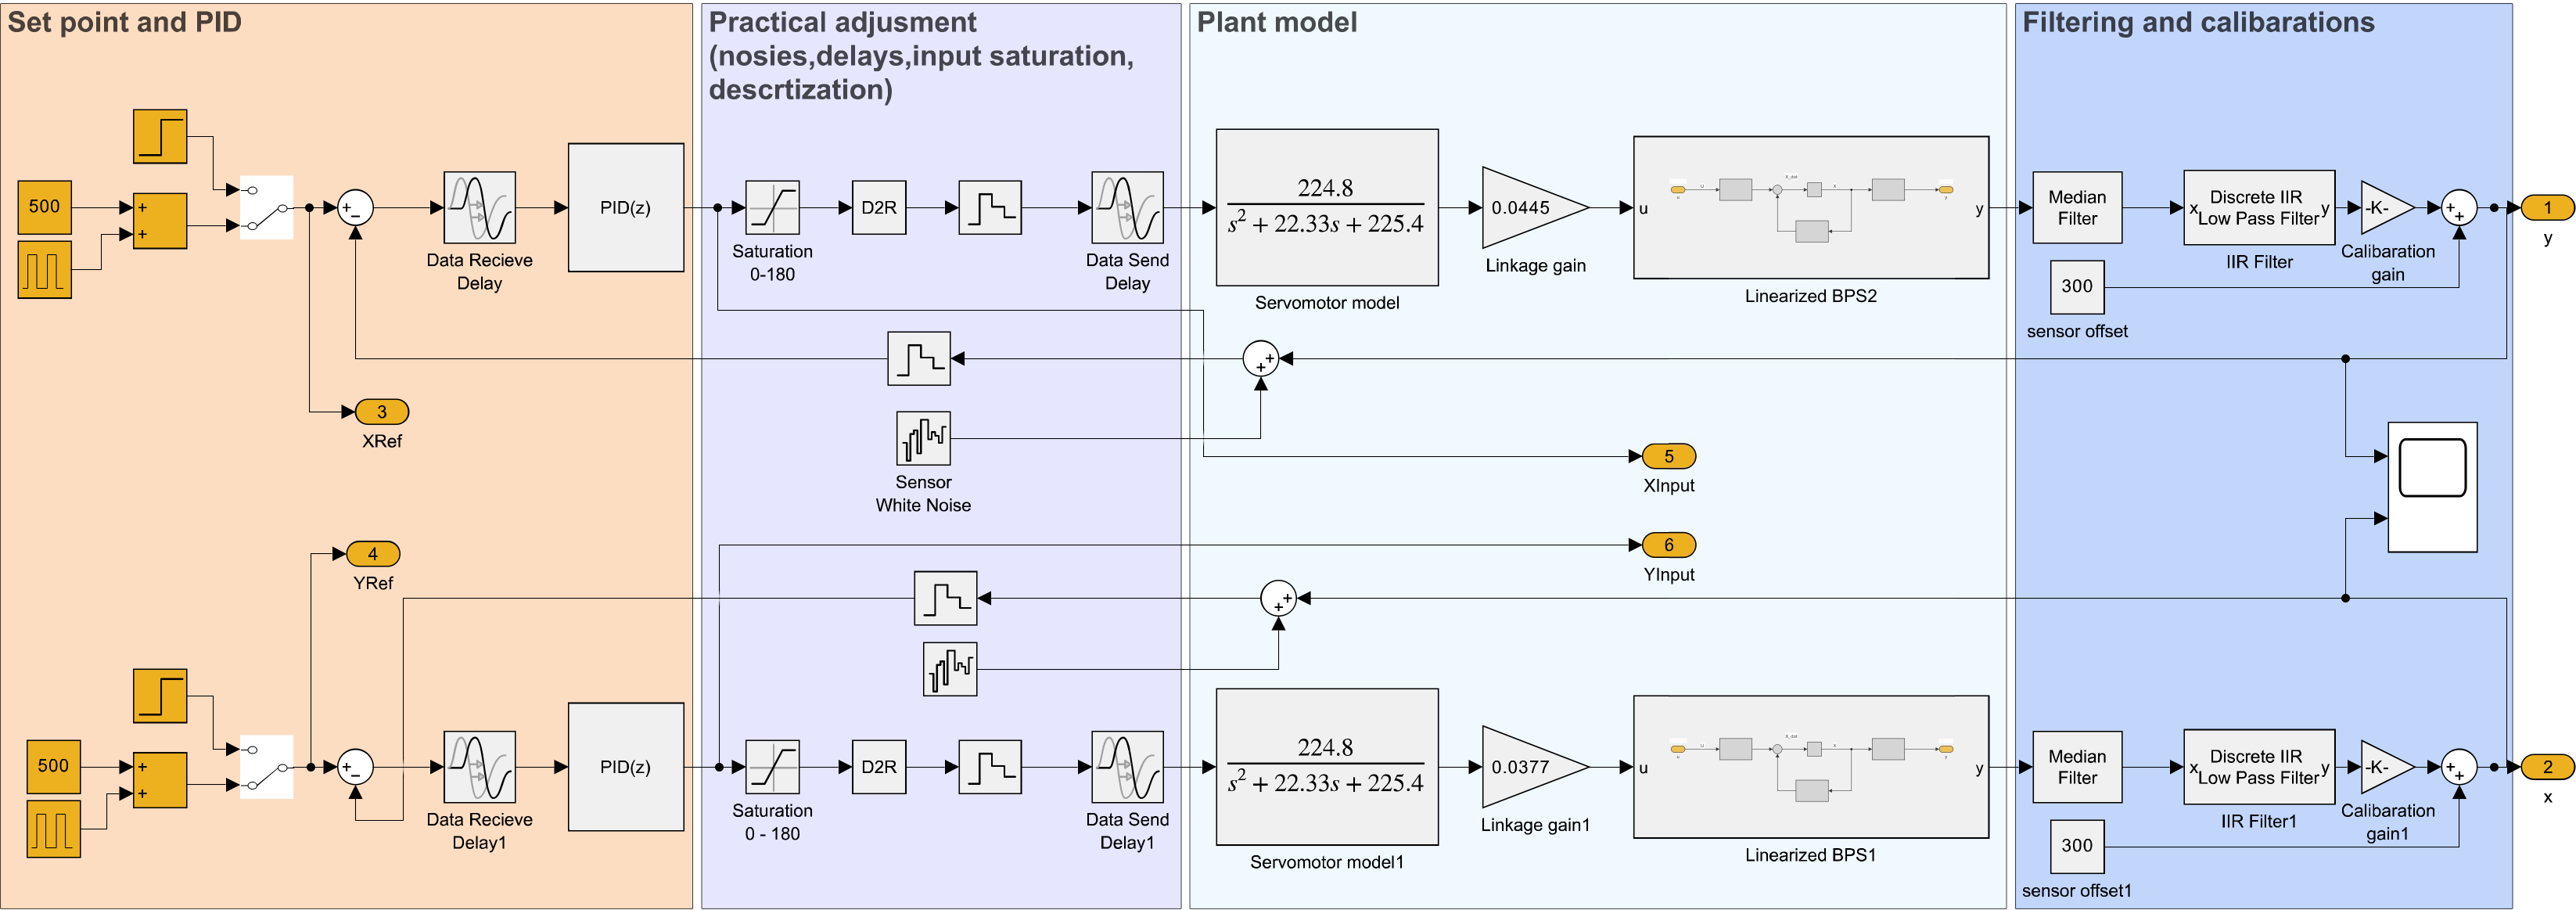
\includegraphics[width=0.95\textheight]{Figures/chapter04/practicalPID.png}
\caption{PID Simulink Model Illustrating Practical Adjustments: saturation, calibration, white noises, communication delays}
\label{fig:IMs matrix correlation}
\end{sidewaysfigure}

\begin{sidewaysfigure}
\centering
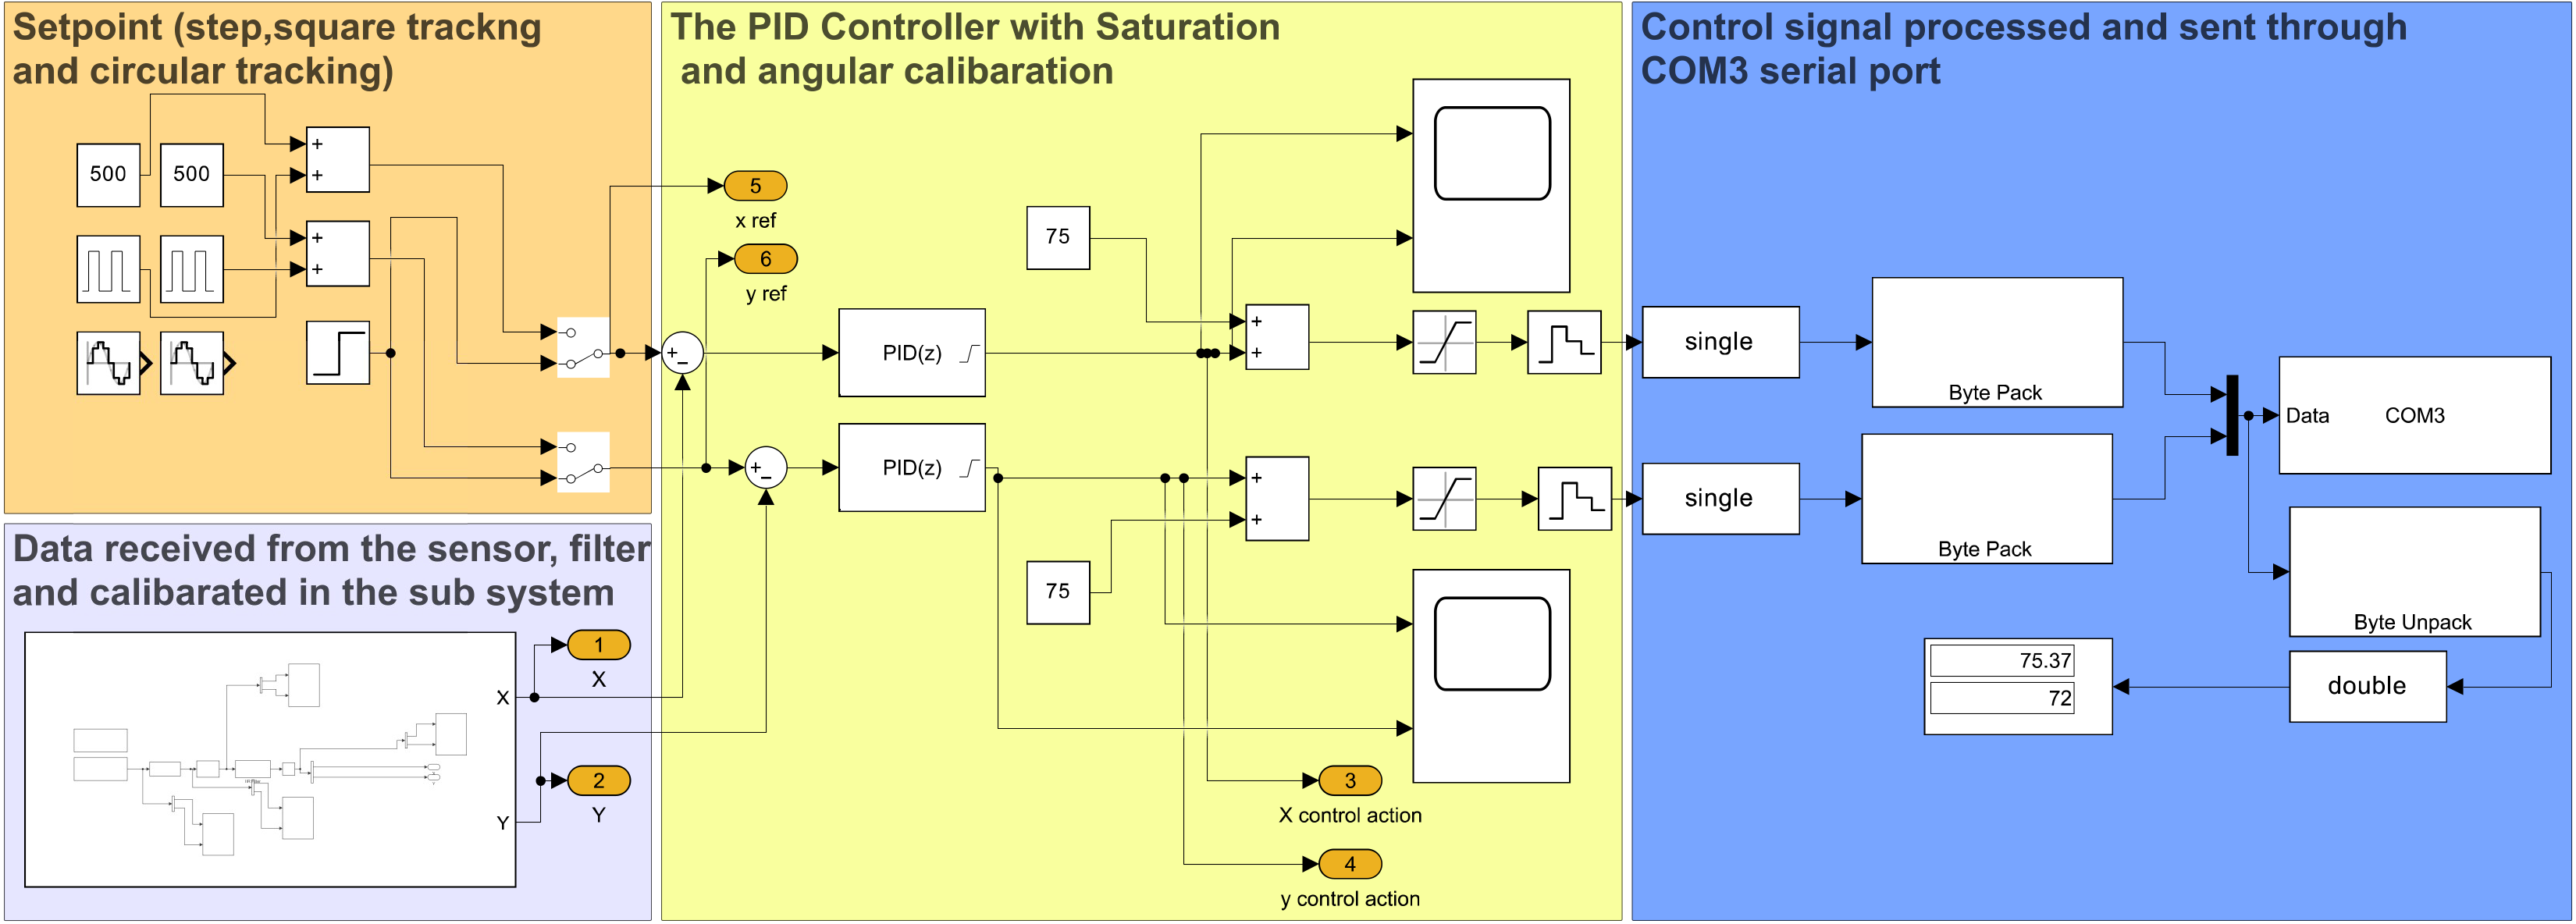
\includegraphics[width=0.95\textheight]{Figures/chapter04/simulink_real_system_pid_model.png}
\caption{Simulink Model used for Controlling the real system}
\label{fig:IMs matrix correlation}
\end{sidewaysfigure}

\begin{sidewaysfigure}
\centering
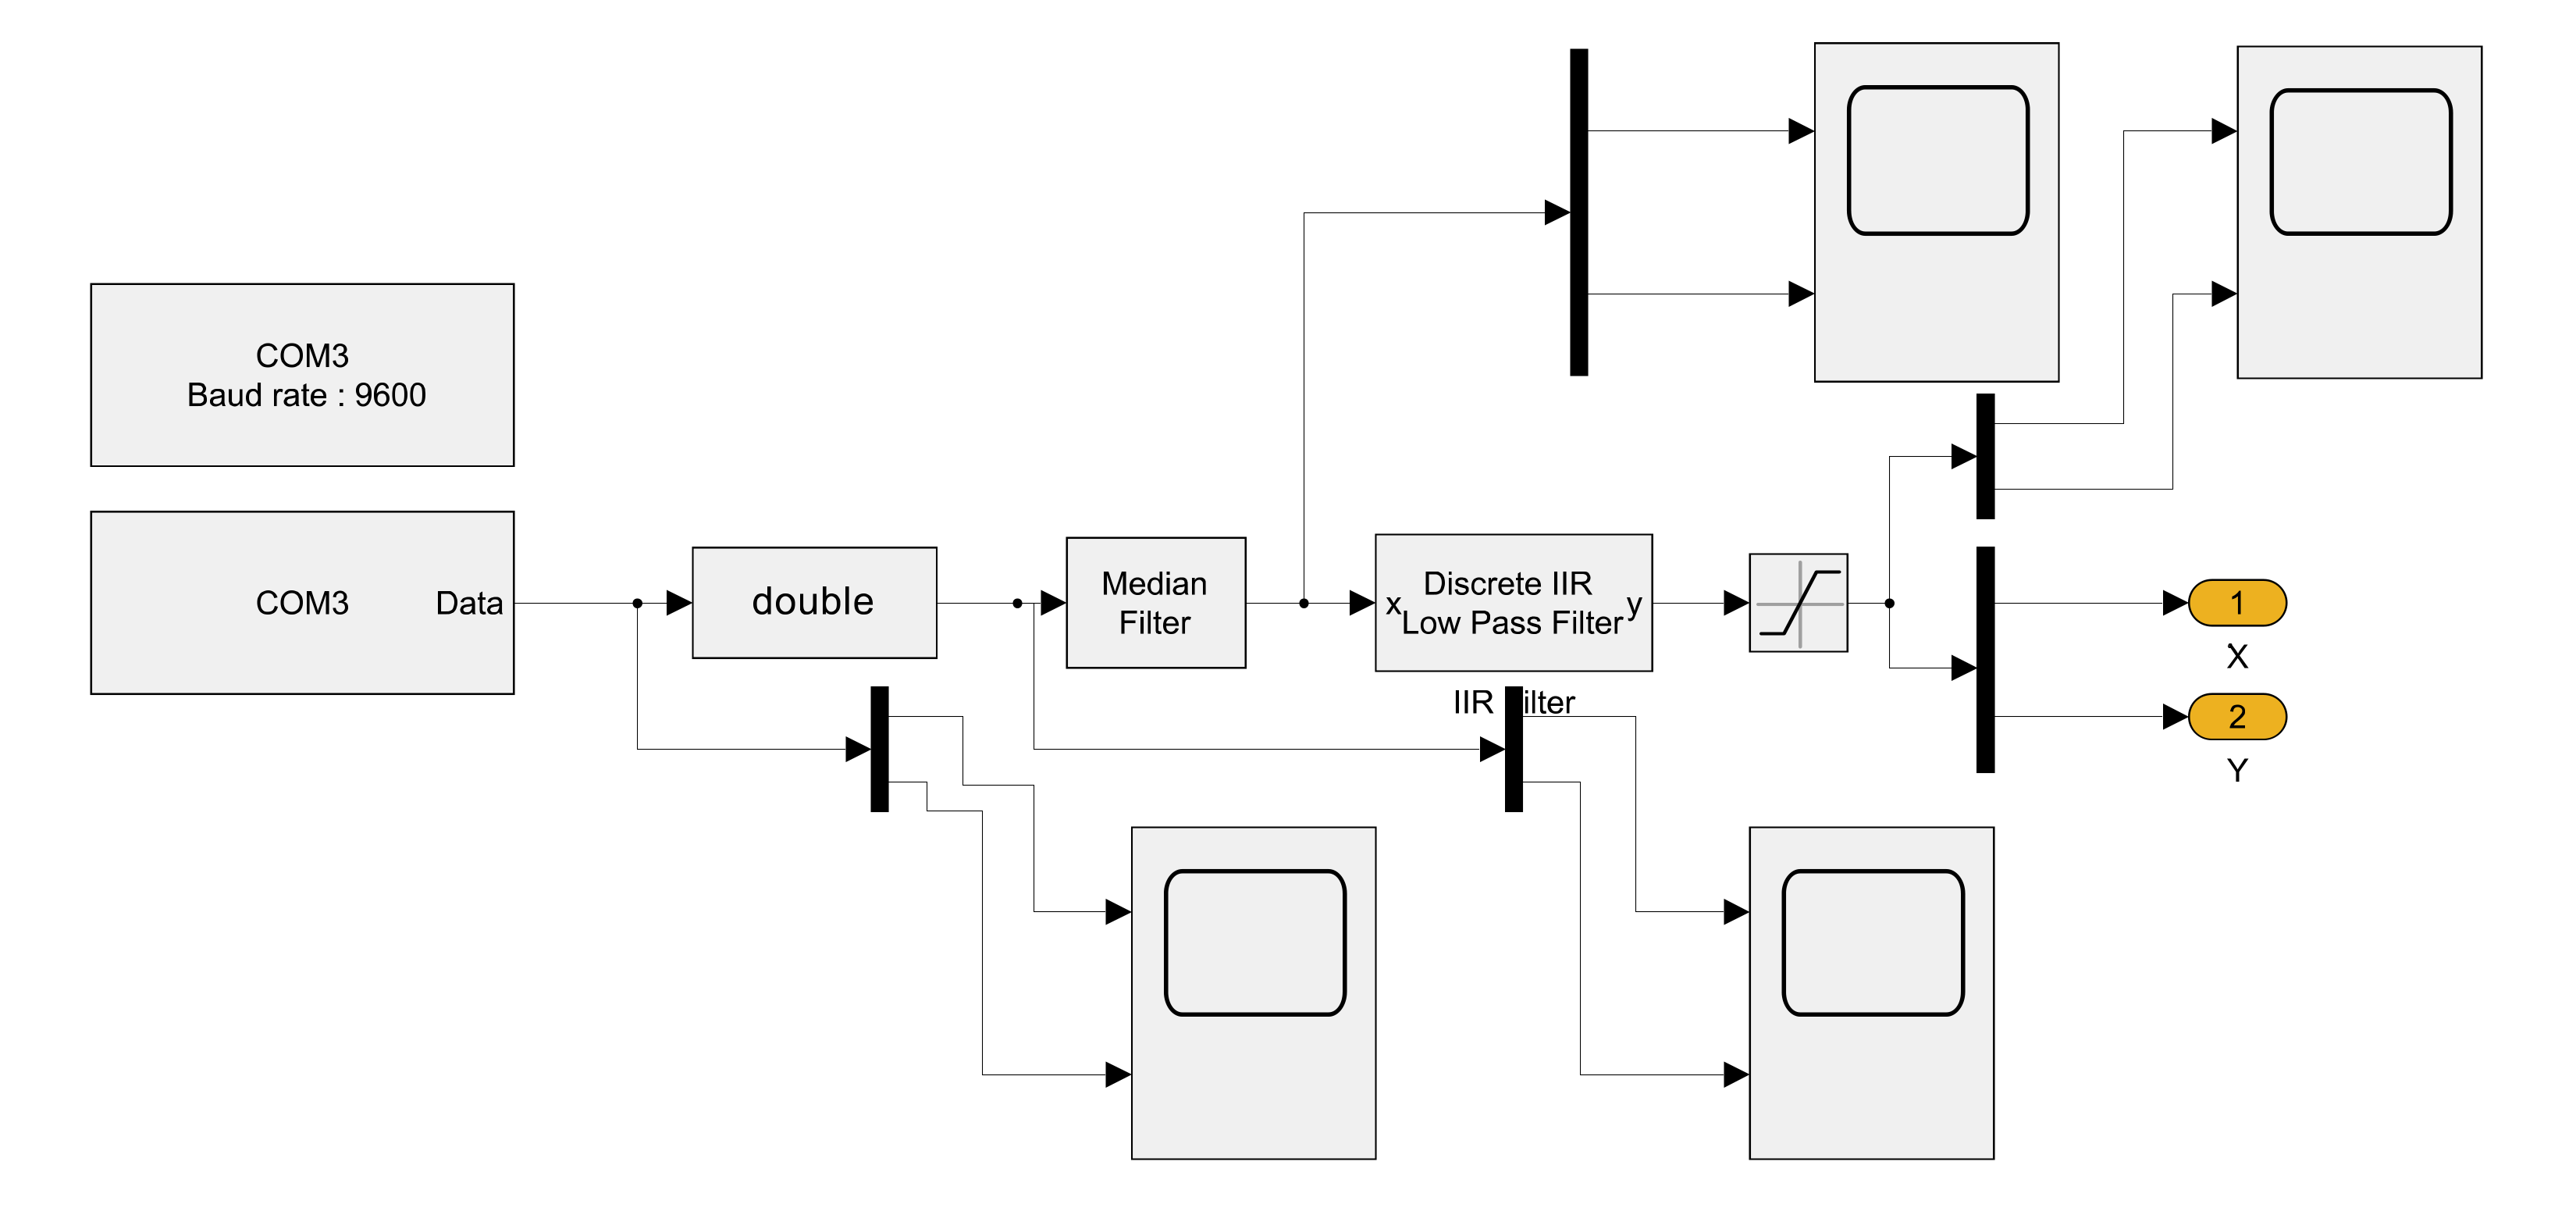
\includegraphics[width=0.85\textheight]{Figures/chapter04/simulink_real_system_pid_model_subsys.png}
\caption{Simulink Block used for receiving the feedback data}
\label{fig:IMs matrix correlation}
\end{sidewaysfigure}
